\documentclass{article}
\usepackage{graphicx}
\usepackage[margin=1.5cm]{geometry}
\usepackage{amsmath}
\usepackage{hyperref}

\begin{document}

\title{Week 12 Writing Activity: Writing Mechanics in Essays and Articles and Chapter 8 of \textit{The Scientific Attitude}}
\author{Prof. Jordan C. Hanson (INTD100)}

\maketitle

\section{Organization and Structure of Scientific Writing}

In Fig. \ref{fig:1}, we encounter an outline of the story of cold fusion.  The trouble is, the ideas are not connected or organized in a way that would lead to a well-constructed scientific essay.  Your task is to reconstruct the outline using the blocks in Fig. \ref{fig:1}.  Note that this means making judgement calls about (a) the proper hierarchy of ideas, and (b) the proper categories or branches for ideas.  Draw your solution on the back of the page.

\begin{figure}[hb]
\centering
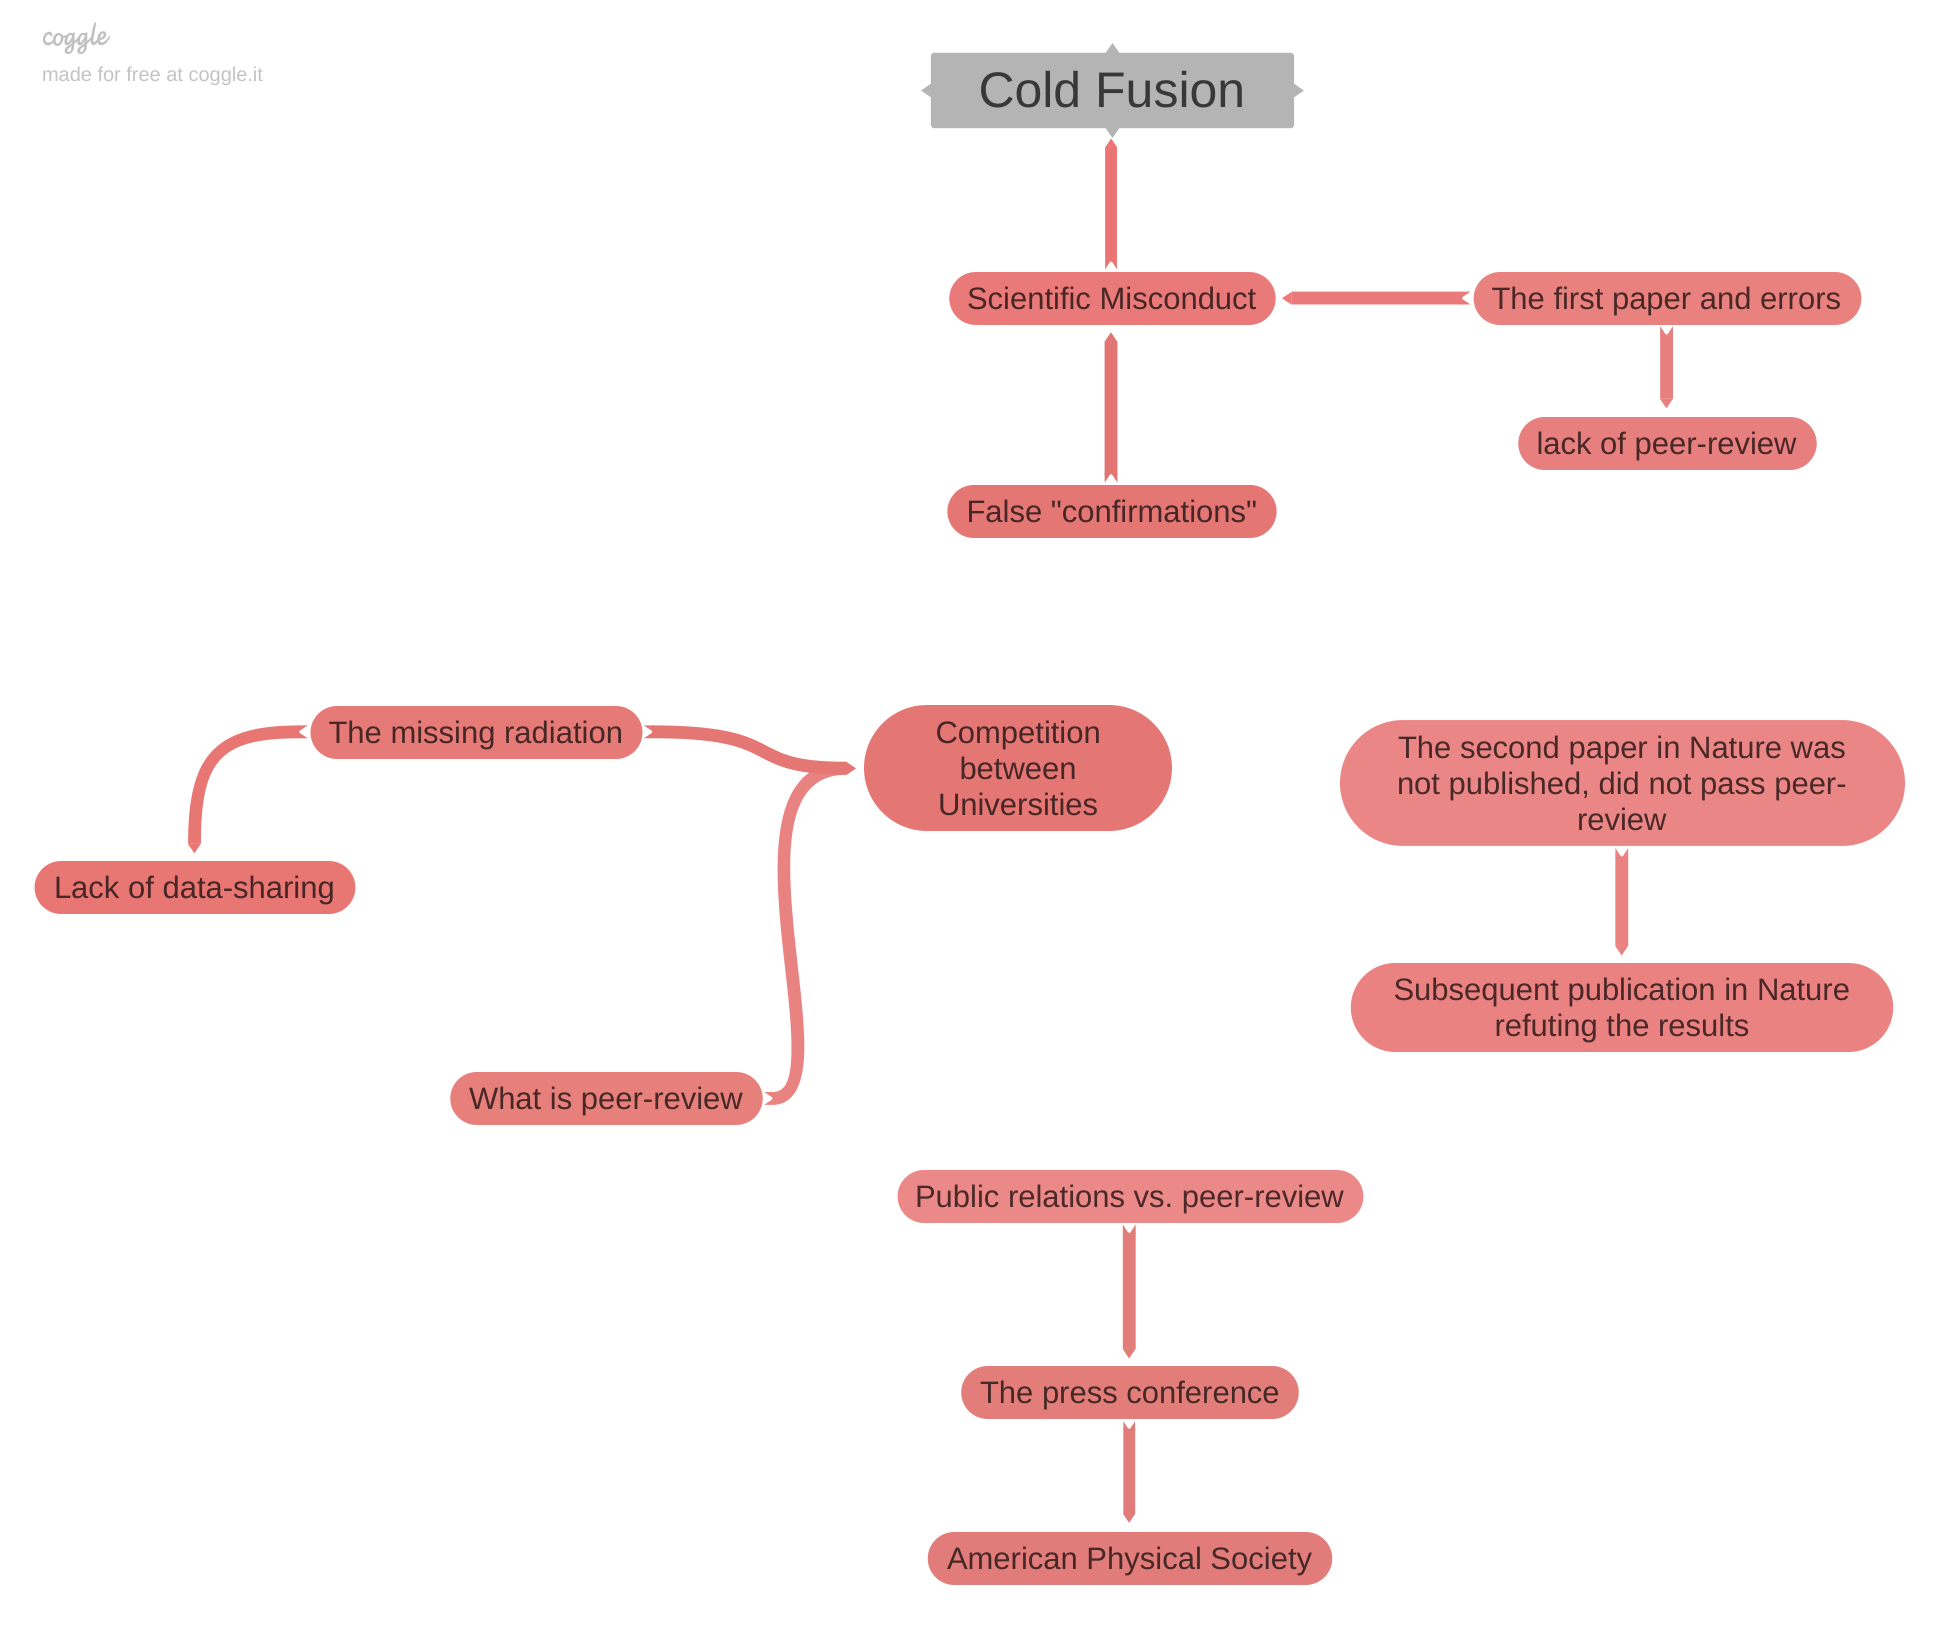
\includegraphics[width=0.8\textwidth]{figures/Cold_Fusion.png}
\caption{\label{fig:1} A partially constructed outline for the story of cold fusion.}
\end{figure}

\end{document}
